\documentclass[journal, a4paper]{IEEEtran}
\usepackage{graphicx}   
\usepackage{url}  
\usepackage{multirow}  
\usepackage{amsmath, verbatim}  
\usepackage[labelfont=sc]{caption}
\usepackage[brazil]{babel}
\usepackage[utf8]{inputenc, color}
\usepackage[T1]{fontenc}
\usepackage{float}
\usepackage{tabularx,ragged2e,booktabs,caption}
\newcolumntype{C}[1]{>{\Centering}m{#1}}
\renewcommand\tabularxcolumn[1]{C{#1}}
% Your document starts here!
\begin{document}

% Define document title and author
	\title{Relatório 2 - Amplificadores CC e BC com TBJ}
	\author{Arthur Pimentel e Matheus Farias}
	\maketitle

    \section{Exercícios}
    	   
        \subsection{Exercício 1}    
            \begin{figure}[H]
        		\begin{center}
        		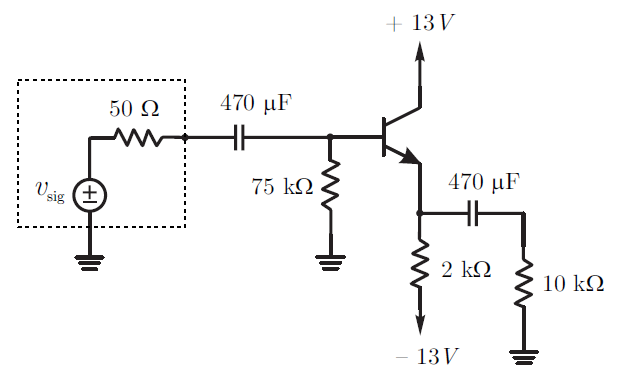
\includegraphics[width=\columnwidth]{CIRCUITO1.png}
        		\caption{Amplificador CC}
        		\label{circuito1}
        		\end{center}
        	\end{figure}
            
            \begin{figure}[H]
        		\begin{center}
        		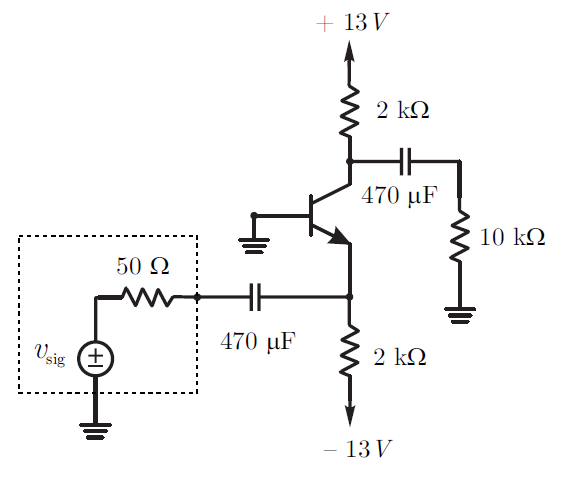
\includegraphics[width=\columnwidth]{circuito2.png}
        		\caption{Amplificador BC}
        		\label{circuito2}
        		\end{center}
        	\end{figure}  
            
            \begin{figure}[H]
        		\begin{center}
        		\caption{Tabela 1}
        		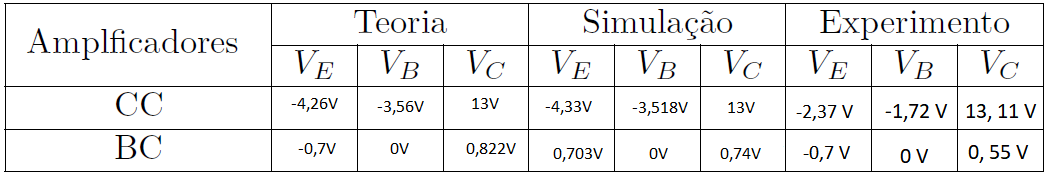
\includegraphics[width=\columnwidth]{tabela11.png}
        		\label{tabela1}
        		\end{center}
        	\end{figure}  
            
            \begin{figure}[H]
        		\begin{center}
        		\caption{Tabela 2}
        		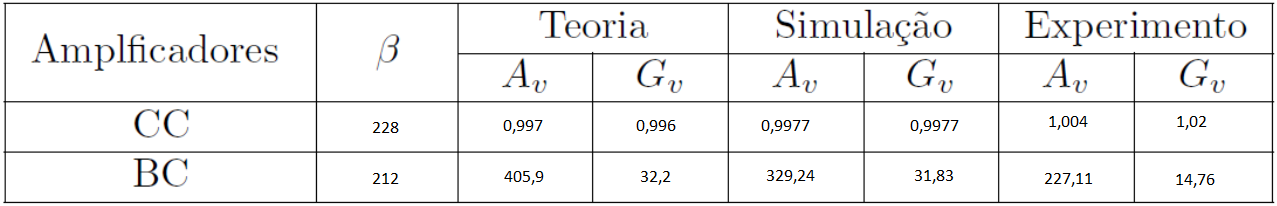
\includegraphics[width=\columnwidth]{tabela12.png}
        		\label{tabela2}
        		\end{center}
        	\end{figure}  
        
        \subsection{Exercício 2}
            \subsubsection{Questão 1} 
                Por análise c.c:
                $$V_C = 13V$$
                $$82kI_B + 0,7 + (\beta +1)2kI_B= 13 \xrightarrow{} I_B=43,3\mu A$$
                $$I_C = \beta I_B = 4,33mA$$
                $$I_E = (\beta +1)I_B = 4,37mA$$
                $$\frac{V_E + 13}{2} = 4,37 \xrightarrow{} V_E = -4,26V$$
                $$V_B = V_E + 0,7 = 3,56V$$
                Por análise c.a usando o modelo T:
                $$r_e = \frac{V_T}{I_E} = 5,72 \Omega$$
                $$10k//2k = 1,66k\Omega$$
                $$A_v = \frac{1,66k}{1,66k + 5,72} = 0,997$$
                $$G_v = A_v \frac{v_i}{v_{sig}} \xrightarrow{} \frac{v_i}{v_{sig}} = \frac{R_{in}}{R_{in} + R_{sig}}$$
                $$R_{in} = 82k//(\beta +1)(5,72 + 10k//2k) = 55,2k\Omega$$
                $$G_v = 0,996$$
            \subsubsection{Questão 2}
                Por análise c.c:
                $$V_B = 0$$
                $$V_E = -0,7 \xrightarrow{} I_E = \frac{-0,7 + 13}{2} = 6,15mA$$
                $$I_B = \frac{I_E}{\beta +1} = 60,89 \mu A$$
                $$I_C = \beta I_B = 6,089 mA$$
                $$\frac{13-V_C}{2}=6,089 \xrightarrow {}V_C = 0,822 V$$
                Por análise c.a usando o modelo T:
                $$v_0 = - \alpha i_e (2k // 10k)$$
                $$i_e = \frac{v_i}{r_e} \xrightarrow{} r_e = \frac{25}{6,15} = 4,065 \Omega$$
                $$A_v = \frac{v_0}{v_i} = \frac{\alpha (2k//10k)}{r_e}$$
                $$A_v = 405,9$$
                $$G_v = A_v \frac{R_{in}}{R_{in}+R_{sig}} \xrightarrow{} R_{in} = 2k//4,06 = 4,05\Omega$$
                $$G_v = 405,9\frac{4,05}{4,05 + 47} = 32,2$$
        \subsection{Exercício 3}
            \begin{figure}[H]
                \begin{center}
                \caption{Circuito 1}
                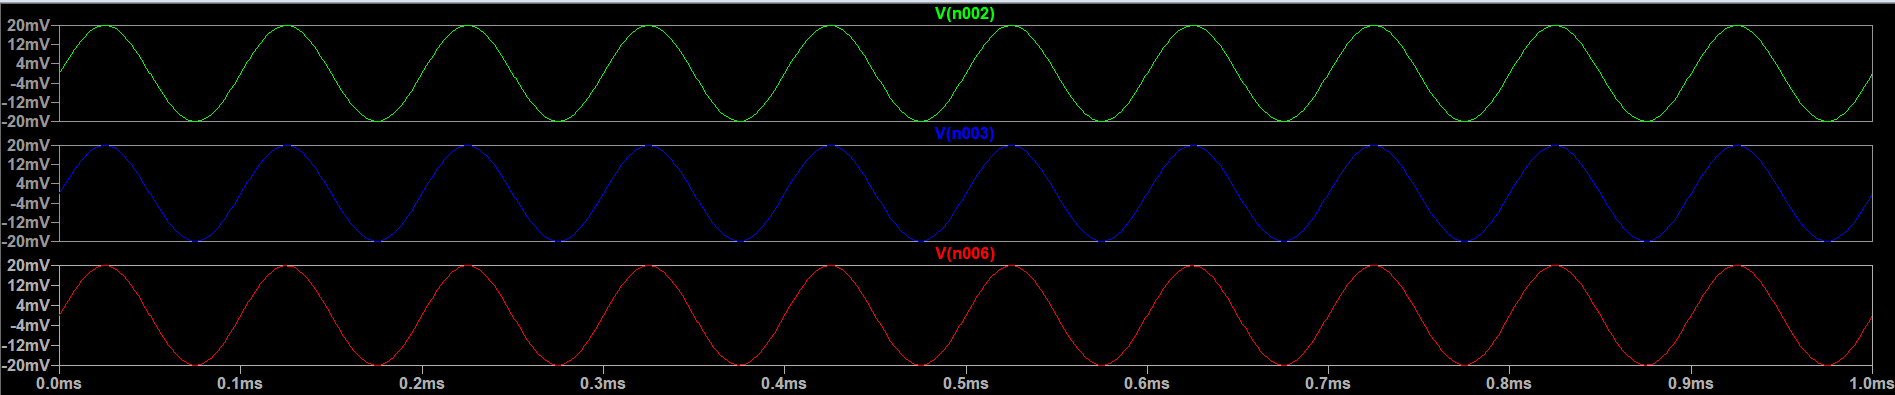
\includegraphics[width=\columnwidth]{vsig1.png}
                \label{tabela2}
                \end{center}
            \end{figure}  
            \begin{figure}[H]
        		\begin{center}
        		\caption{Medições do Circuito 1}
        		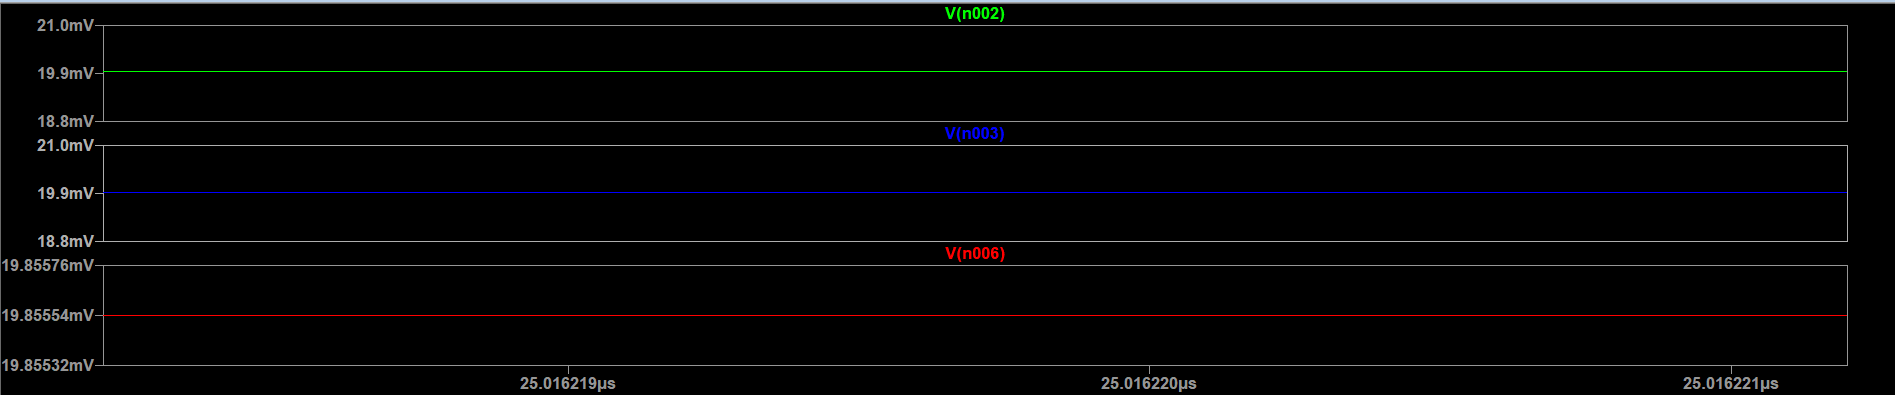
\includegraphics[width=\columnwidth]{mede1.png}
        		\label{tabela2}
        		\end{center}
            \end{figure}  
            \begin{figure}[H]
        		\begin{center}
        		\caption{Circuito 2}
        		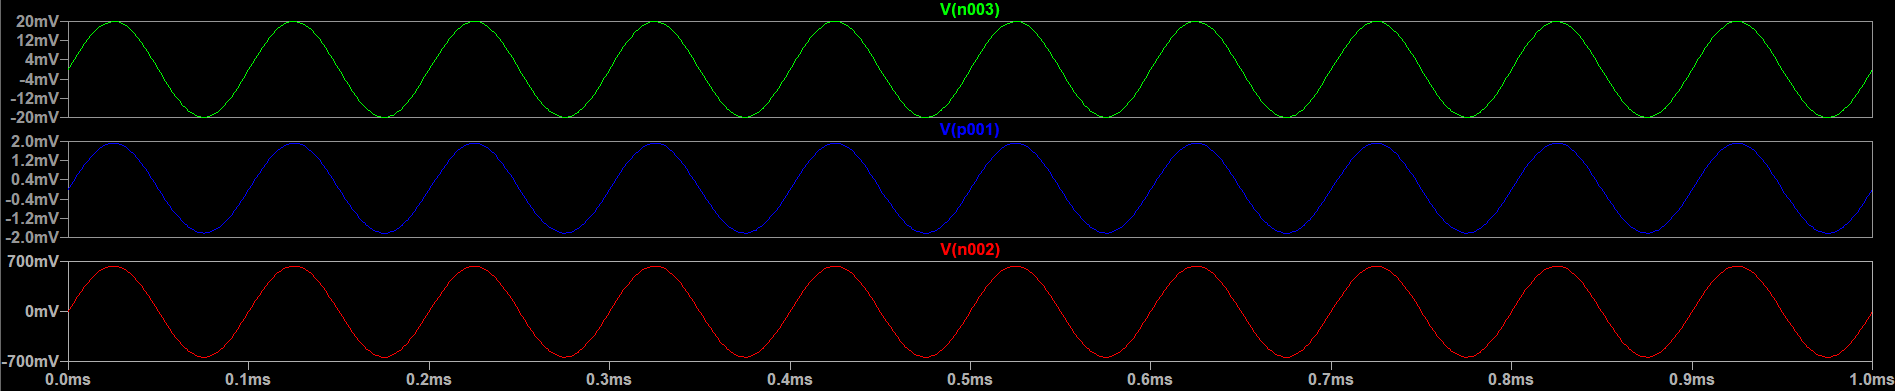
\includegraphics[width=\columnwidth]{vsig2.png}
        		\label{tabela2}
        		\end{center}
            \end{figure}  
            \begin{figure}[H]
        		\begin{center}
        		\caption{Medições do Circuito 2}
        		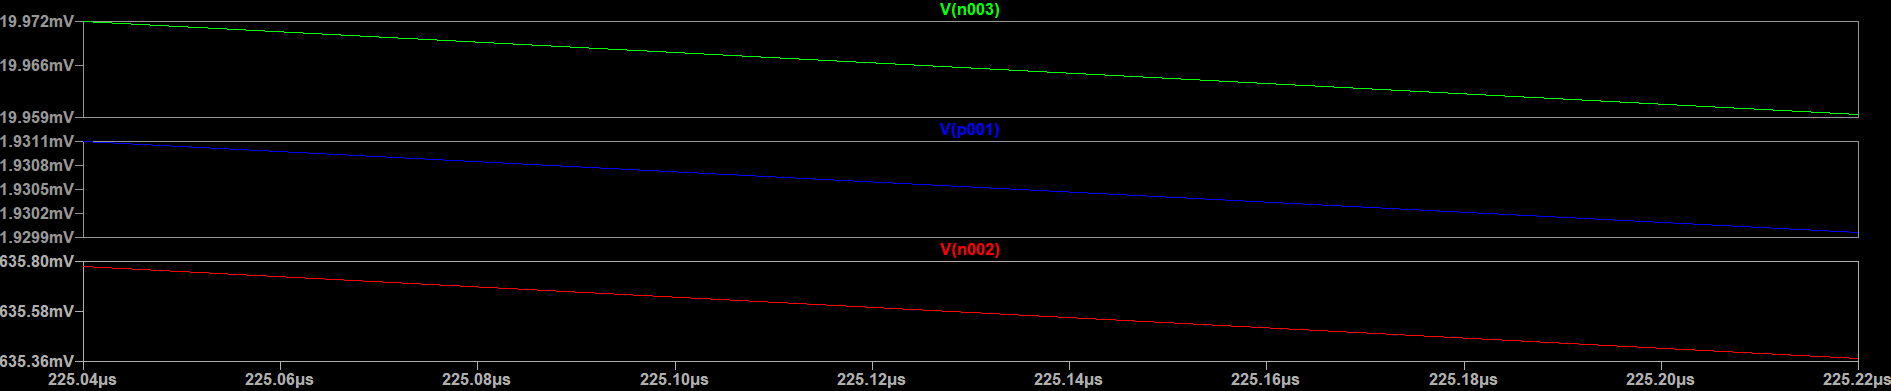
\includegraphics[width=\columnwidth]{mede2.png}
        		\label{tabela2}
        		\end{center}
        	\end{figure}   
        \subsection{Exercício 4}
            \begin{figure}[H]
        		\begin{center}
        		\caption{Amplificador CC}
        		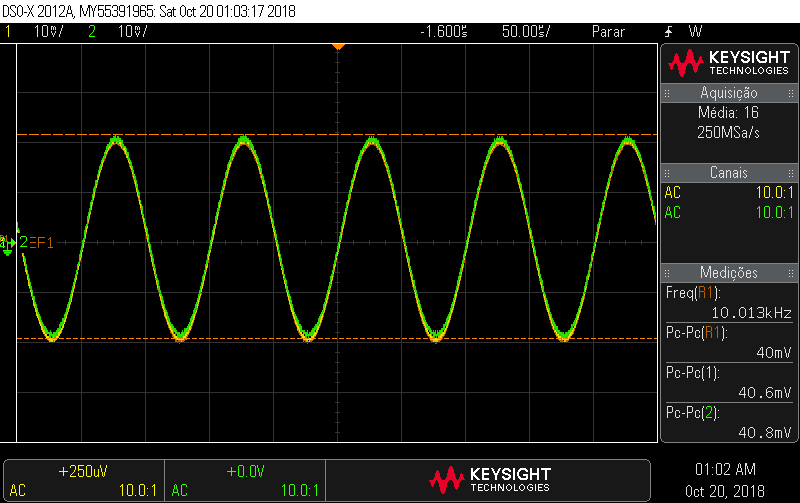
\includegraphics[width=\columnwidth]{scope_0.png}
        		\label{scope0}
        		\end{center}
        	\end{figure}

            \begin{figure}[H]
        		\begin{center}
        		\caption{Amplificador BC}
        		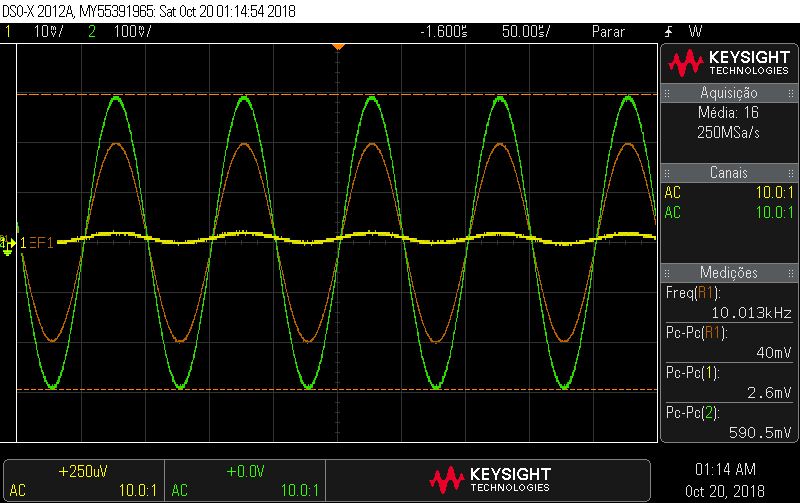
\includegraphics[width=\columnwidth]{scope_1.png}
        		\label{scope1}
        		\end{center}
        	\end{figure}        
          \subsection{Exercício 5}
    			Na maioria dos casos o resultado foi parecido, porém, primeiramente, é importante ressaltar que na análise teórica foi utilizado o valor de $\beta$ sendo $100$, enquanto na prática os valores foram praticamente o dobro. Depois, na análise teórica, os modelos de pequenos sinais são feitos usando o fato que os capacitores têm capacitância infinita, que obviamente não é o caso da prática. E por último, a análise de pequenos sinais toma como base a relação $V_{sig} \ll V_T$, onde $V_T = 25$mV é a tensão térmica à temperatura do laboratório, como o sinal trabalhado não é muito menor que a tensão térmica, surgem erros de análise. Além disso tem-se, claro, os erros corriqueiros, como a tolerância do resistor, a variação de sua resistência com a temperatura, imperfeições da protoboard, etc.
			
\end{document}